%%This is a very basic article template.
%%There is just one section and two subsections.
\documentclass{main}
 

\usepackage{graphicx}      % include this line if your document contains figures
\usepackage{natbib}        % required for bibliography
\usepackage{subfigure}
\usepackage{enumerate}
\usepackage[utf8]{inputenc}
\usepackage{graphicx}
\usepackage{caption}
\usepackage{subcaption}

\begin{document}

\begin{frontmatter}

\title{Robôs para Metalização por Chama de Alta Velocidade (HVOF) de palhetas de
turbinas hidráulicas: estudo do estado da arte
\thanksref{footnoteinfo}} 

\thanks[footnoteinfo]{This work is supported by ESBR under contract COPPETEC
JIRAU 151/13 6631-0002/2013 (ANEL R\&D program).}

\author[1]{Renan S. Freitas}
\author[1]{Gabriel Alcantara C. S.}
\author[1]{Eduardo Elael M. S.}
\author[1]{Ramon R. Costa}
\author[2]{Sylvain Joyeux}
\author[2]{Patrick M. Paranhos}

  \address[1]{Departamento de Engenharia Elétrica, COPPE UFRJ, Rio de Janeiro,
  Brasil} 
 %TODO
  \address[2]{Centro de Inovação em Robótica (CIR), Rio de Janeiro, Brasil}
 
\begin{abstract}                % Abstract of not more than 250 words.
%TODO 
\end{abstract} 

\begin{keyword}
%TODO
\end{keyword}

\end{frontmatter}

\section{Introdução}
%TODO Renan: Introdução
Hydropower is the most mature, reliable and cost-effective
renewable power generation technology available \citep{brown}, accouting 16
percent of global electricity generation. The global hydropower use and
capacity will increase about 3.1\% each year for the next 25 years \citep{wi}.
The total investment for large-scale hydropower projects
typically range from USD 1000/kW to around USD 3500/kW and, once commissioned,
the annual operation and maintenance costs of hydropower plants are often
quoted as 4\% of the investment per kW per year \citep{ecofys}. 

In the specific case of Brazil, the third biggest hydroelectric potential of
the world, hydropower represents 84\% of its electric power total production.
Brazil is the second biggest country of installed hydropower capacity, 84 GW,
and in the Amazon basin, in Madeira river, this number will be increased next
years by the construction of Santo Antonio (3150 MW) and Jirau (3300 MW) power
plants. The dependance on this renewable power source mobilizes private
initiative investments on research centers and universities, and motivates the
development systems with a high degree of automation based on advanced robotic
systems \citep{aneel}.

A major challenge for hydropower companies is\ldots


 


In this paper, we present the state of the art in\ldots

%a general overview of the
%ROSA robot, and a detailed description of the embedded electronics, power
% supply system and software architecture. The robot is designed to perform monitoring and inspection
%tasks of the stoplogs' stacking and retrieving process in a power
%plant. Carrying different sensors, the robot analyses sensor data \emph{in
%loco} or stores it for a posterior analysis, interprets the results, and
%sends specific data to the operator. The sensors can identify the lifting beam
%actual operation (stack/retrieve), stoplog attachment/detachment, the
%lifting beam inclination, the system depth in water, and a
%profiling sonar for sediments inspection. 

%This text is organized as follows: the state of the art general overview of the
%robot and its main challenges are presented in Section \ref{sec:sota}, detailed
%descriptions of the embedded electronics, the vehicle support system, power
%supply system, and software architecture are taken in
%Sections \ref{sec:electronics_overview}, \ref{sec:powersupply_overview}, and
%\ref{sec:software} respectively.
%In Section \ref{sec:results}, preliminary results are shown, and concluding
%remarks are drawn in Section \ref{sec:conclusions}.
\section{Descrição do problema}\label{sec:consideracoes}
%TODO Renan: introdução do problema
%TODO Renan: Descrição do processo HVOF (questoes HVOF) e cavitação
%TODO Gabriel: Caso JIRAU/contextualização (Ambiente). Detalhe dos acessos 
%TODO Elael: Tarefas do Robô
O fenômeno de cavitação em hidroturbinas provoca redução da eficiência na
geração de energia e desgaste superficial por erosão. Uma solução preventiva é
o revestimento por metalização das pás, o qual aumenta a eficiência na
geração de energia por gerar uma estrutura mais lamelar, e fornecer maior
resistência a desgastes abrasivos, corrosivos e erosivos.

A cavitação é um fenômeno físico que ocorre quando há quedas repentinas de
pressão. Em uma


\section{Estado da arte}\label{sec:sota}
 
O estudo do estado da arte de robôs para a realização de HVOF em pás de turbinas
hidráulicas contempla os sistemas que atendem a alguns dos requisitos: operar
em ambientes de alta periculosidade; capacidade de carga para os dispositivos HVOF;
manipular a pistola HVOF com velocidade de $0.67 m/s$; precisão de 5mm; ter
área de trabalho de 2.5 m x 2.5 m; e operar sob superfícies 3D de geometria
complexa. As soluções foram divididas em subseções de acordo com as tecnologias
de fixação dos robôs.


 
\subsection{Robôs sobre trilhos}
%TODO características gerais do robo: fixação,
% sensores, sistema HVOF e etc
% aplicação,
% vantagens e desvantagens

%oq sao e motivaçaõ
%teconologias de fixaçaõ
%robos
%vantagems/desvantagens

Na indústria, a automatização de processos de \textit{hard coating},é
normalmente realizada com a utilização de manipuladores robóticos. Esse tipo de
robô proporciona uma versatilidade operações, uma vez que podem ser
reprogramados para realizar tarefas repetidamente com alta precisão. O espaço de
trabalho de um braço robótico é dependente do numero de juntas presentes no
robô, rotacionais ou prismáticas, e pelo tamanho de cada elo. As juntas
determinam os graus de liberdade e mobilidade que um manipulador possuí,
enquanto o tamanho dos elos influenciária no alcane máximo do robô.

Os processos de manunteção de turbinas, como o \textit{hard coating}, exigem a
realização trajetórias complexas, o que siginifica a necessidade de várias
juntas, e o tamanho das pás da turbina exigem que o manipulador tenha um alcance
máximo pelo menos maior que a maior dimensão da pá. Portanto, os manipuladores
robóticos utilizados para esse tipo de aplicação são, geralmente, robôs
industrias que pesam centenas de quilos, com mais de 2 metros de alcance máximo
e necessitam de uma fixação que garantam que o manipulador não irá se movimentar
ao realizar suas tarefas programadas. 

Para a automatização de um processo de manutenção \textit{in-situ} é
necessário, porém, que o sistema projetado seja compacto, de fácil instalação, e
que nâo exija alterações estruturais permanentes para a sua utilização. Um
manipulador robótico convencional que necessite de um espaço de trabalho
suficiente para executar tarafas em toda a superfície da pá de uma turbina se
torna, então, inviável. 

Uma estratégia para reduzir o tamanho e peso de um manipulador robótico é
torná-lo móvel. Isso pode ser alcançado com a introdução de mais uma junta
prismática acoplada a um trilho, possibilitando que o manipulador estenda seu
espaço de trabalho por toda a extensão do trilho.

Na literatura foram encontradas duas soluções para aplicações de manutenção e
inspeção, como solda. As aplicações diferem principalmente na estratégia de
fixação do trilho. O Roboturb \cite{roboturb} realiza a fixação diretamente na
pá do rotor, enquanto o robô Scompi \cite{scompi} utiliza uma fixação exterior 



\subsection{Robôs escaladores}
%TODO características gerais do robo: fixação,
% sensores, sistema HVOF e etc
% aplicação,
% vantagens e desvantagens
Robôs escaladores são sistemas capazes de sustentar seu próprio peso contra a
gravidade, movendo-se em simples ou complexas estruturas geométricas, como
paredes, tetos e telhados, palhetas de turbinas e plantas nucleares.
Essa classe de robôs oferece eficiência operacional em ambientes
de alta periculosidade, sendo utilizados visando saúde e segurança dos
trabalhadores, como em inspeção e limpeza de arranha-céus, diagnóstico de
tanques de armazenamento em plantas nucleares, solda e manutenção de cascos de
navios e palhetas de turbinas \cite{clawar}.

Os grandes desafios nos projetos de sistemas escaladores são mobilidade e
aderência, além de consumo de energia, capacidade de carga e peso. Em
\cite{modular}e \cite{climbsurv}, os robôs escaladores são divididos em tipos de locomoção:
pernas, como andador, utilizando segmentos deslizantes, rodas, esteiras, avanço
pendurado por braços, por cabos e biomimética; e categorias de adesão: sucção ou
pneumática, magnética, eletrostática, química, preensão e híbrida.

No caso específico deste estudo da arte, destacam-se os robôs escaladores com as
seguintes aplicações:

\begin{itemize}
  \item \emph{Construção de navios e turbinas}: RRX3 para soldagem
  \citep{rrx3}, \emph{Climbing Robot for Grit Blasting} para limpeza
  \citep{crgb} e ICM Robot para inspeção \citep{icm};
  \item \emph{Construção industrial}: ROMA II \citep{roma} e
  CROMSCI \citep{CROMSCI}, ambos para inspeção; 
 \item \emph{Planta petroquímica}: ROBICEN \citep{robicen} e
  TRIPILLAR \citep{tripillar}, ambos para inspeção.  
\end{itemize}

O RRX3 é um robô para a soldagem de casco de navios. Possui adesão por
preensão, locomoção transversal utilizando segmentos deslizantes e locomoção
longitudinal por rodas. Possui um manipulador de 1.5 m com três juntas
prismáticas e três juntas de revolução (3P3R) para a operação de soldagem. Suas
principais vantagens e desvantagens em relação à aplicação HVOF são:

\textbf{Vantagens:}
\begin{itemize}
  \item Base com capacidade de carga 120 kg;
  \item Manipulador com capacidade de carga 5 kg;
  \item Manipulador de precisão milimétrica;
  \item Robô robusto que trabalha com instrumento de alta temperatura (solda);
\end{itemize}

\textbf{Desvantagens:}
\begin{itemize}
  \item Locomoção restrita impede utilização em estruturas geométricas
  complexas;
  \item Manipulador não possui alcance suficiente para a aplicação fim;
  \item Manipulador com efetuador de baixa velocidade;
\end{itemize}

O \emph{Climbing robot for Grit Blasting} é um robô para jateamento abrasivo em
navios. O robô utiliza duas plataformas deslizantes com sistema de adesão por
ímã magnético. Os módulos apresentam movimentação relativa entre si e pode rotar
para compensar as curvaturas do casco do navio ou desviar de objetos. 

\textbf{Vantagens:}
\begin{itemize}
  \item Base com capacidade de carga de sistema abrasivo semelhante ao HVOF;
  \item Base com locomoção de precisão milimétrica;
\end{itemize}

\textbf{Desvantagens:}
\begin{itemize}
  \item Locomoção ampla, porém não aplicável às estruturas geométricas
  complexas. A curvatura do casco é simples quando comparada à pá da turbina;
  \item Não possui manipulador, logo o sistema deve percorrer todo o
  casco;
  \item A instalação de um manipulador prejudica a estabilidade do sistema;
\end{itemize}

\emph{The Climber}, ICM Robotics, é um robô para inspeção de turbinas eólicas,
remoção de revestimento, limpeza de superfície, e aplicação de revestimento.
Possui adesão pneumática (sucção) e locomoção por esteiras. 

\textbf{Vantagens:}
\begin{itemize}
  \item Base com capacidade de carga de 25 kg;
  \item Base com locomoção de precisão milimétrica;
  \item Manipulador para revestimento HVOF pode ser acoplado à base; 
\end{itemize}

\textbf{Desvantagens:}
\begin{itemize}
  \item Manipulador com baixo alcance;
  \item Manipulador com efetuador de baixa velocidade;;
  \item Locomoção apresenta restrição a certas curvaturas devido às esteiras;
\end{itemize}

O ROMA II, Universidade Carlos II de Madrid, é um robô para inspeção de
ambientes complexos. A sua tecnologia de adesão é pneumática (sucção) e
locomove-se como uma lagarta (biomimética). Sua movimentação e planejamento de
trajetória são realizados de maneira ótima de forma a garantir estabilidade e
evitar obstáculos. 

\textbf{Vantagens:}
\begin{itemize}
  \item Base com grande capacidade de carga;
  \item Base com locomoção de grande precisão;
  \item Movimenta-se em ambientes de grande complexidade geométrica; 
\end{itemize}

\textbf{Desvantagens:}
\begin{itemize}
  \item Não possui manipulador para aplicação HVOF;
  \item A instalação de um manipulador irá desequilibrar o sistema,
  principalmente durante a locomoção;
\end{itemize}


CROMSCI, Kaiserslautern University of Technology, é um robô autônomo para
inspeção de grandes paredes de concreto, como pilares de pontes, barragens. Seu
sistema de adesão é composto por sete câmaras de vácuo (sucção), com um sistema
de controle por válvulas e sensores de pressão para reagir rapidamaente a
condições adversas. Locomove-se com rodas omnidirecionais para locomoção.

\textbf{Vantagens:}
\begin{itemize}
  \item Base com locomoção de precisão milimétrica; 
\end{itemize}

\textbf{Desvantagens:}
\begin{itemize}
  \item Manipulador com alcance de 80 cm;
  \item Manipulador com efetuador de baixa velocidade;
  \item Protótipo ainda com pouca capacidade de carga;
\end{itemize}

Planta petroquímica: ROBICEN

TRIPILLAR, École polytechnique fédérale de Lausanne, é um robô escalador de
pequeno porte (96 x 46 x 64 mm) desenvolvido para a inspeção de plantas
petroquímicas. Utiliza um sistema como pernas de lagarta magnéticas em um
formato triangular. Locomove-sepor esteiras.

\textbf{Vantagens:}
\begin{itemize}
  \item Base com locomoção de precisão milimétrica;
  \item Sistema robusto;
  \item Controle simples;
  \item Pequenas dimensões; 
\end{itemize}

\textbf{Desvantagens:}
\begin{itemize}
  \item Não foi testado em estruturas de grande complexidade geométrica; 
  \item Não apresenta manipulador;
  \item Protótipo ainda com pouca capacidade de carga;
\end{itemize}
   

\subsection{Robôs Cabeados}
% 1 OQ SAO, MODTIVACAO
% 2 TECNOLOGIA DE FIXACAO
% 3 NOSSOS ROBOS
% Vantagens e desvantagens
%TODO características gerais do robo: fixação,
% sensores, sistema HVOF e etc
% aplicação,
% vantagens e desvantagens

São classificados como robôs cabeados quaisquer sistemas robôticos que façam
uso de um conjunto de cabos e/ou cordas para auxiliar ou mesmo garantir seu
posicionamento adequado na sua região de trabalho. Sendo assim, robôs cabeados
podem possuir outros métodos de fixação em conjunto com seu cabeamento.

A idéia do uso de um sistema de cabos surge naturalmente, quando o deslocamento
se mostra majoriamente restrito a um plano vertical e não há exigência de
grandes velocidades de deslocamento, como forma de reduzir o preso e melhorar o
desempenho de um braço mecânico de mesmo alcance, ou diminuir a complexidade e
a força de aderência necessária para um \textit{crawler}.



\subsection{Manipulador com base esférica}
%TODO características gerais do robo: fixação,
% sensores, sistema HVOF e etc
% aplicação,
% vantagens e desvantagens
Um projeto de pesquisa e desenvolvimento foi apresentado em
\cite{motta2010prototype} com o objetivo de propor metodologia, simulação e
os passos para construção de um sistema robótico para recuperar danos materiais
em pás de turbinas hidráulicas gerados devido à cavitação. O sistema robótico faz
reparo utilizando a tecnologia de soldagem a arco elétrico, antes realizada
manualmente em ambientes de alta periculosidade com temperaturas que variam
entre $40^o C$ e $99^o C$ em operações que duram em torno de 10 horas.

O robô deve atender aos seguintes requisitos:
\begin{itemize}
  \item Capacidade de operar em qualquer posição: horizontal, vertical,
  invertida;
  \item Pouco peso para portabilidade e fixação às pás;
  \item Rigidez à deflexão: carga no punho do manipulador ocorre em qualquer
  direção e extensão;
  \item Grande precisão na mobilidade;
  \item Disponibilidade de peças no mercado;
  \item Controle com interface de usuário;
  \item Grande área de trabalho;
  \item Facilidade de adesão às pás de turbinas hidráulicas.
\end{itemize}

A solução para o sistema robótico apresenta topologia esférica, como pode ser
visto na figura~\ref{fig:esferico} e características:

\begin{figure}[ht]
\centering
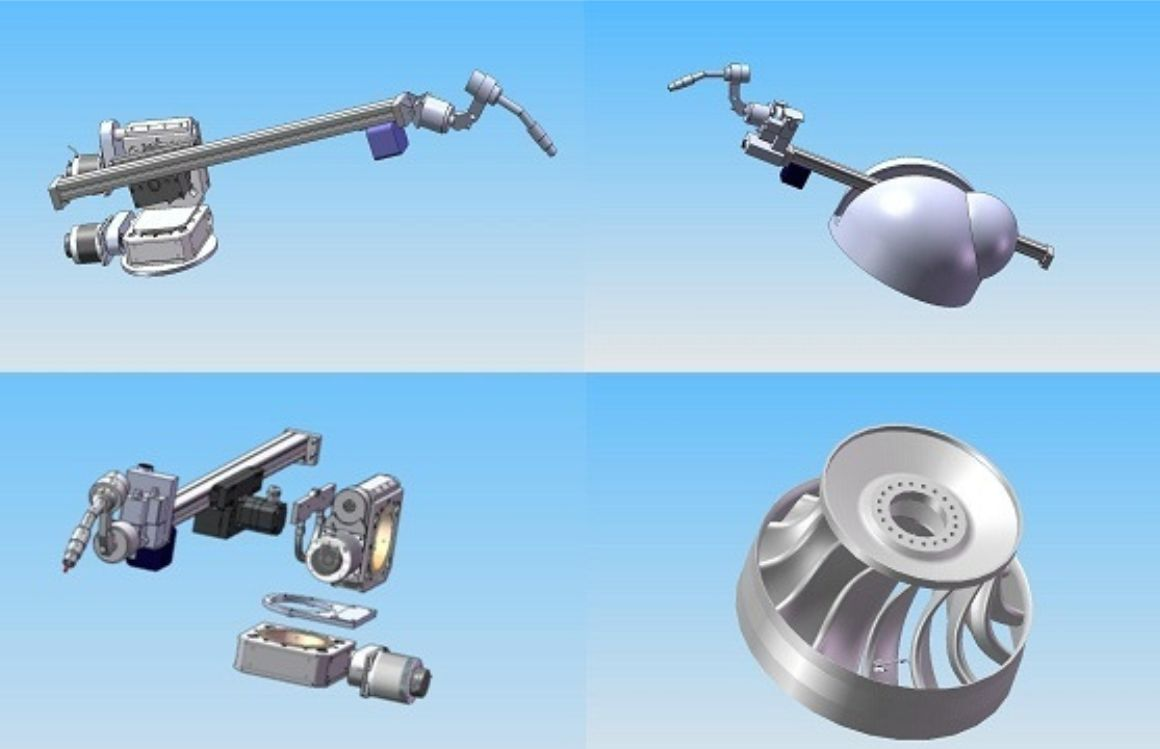
\includegraphics[width=8.4cm]{figs/esferico/esferico.jpg}
\caption{Ilustração do projeto do manipulador com base esférica.}
\label{fig:esferico}
\end{figure}

\begin{itemize}
  \item Três (3) graus de liberdade no manipulador (2R1P) e dois graus de
  liberdade no punho (2R);
  \item Mapeamento de superfície 3D com laser;
  \item Eletrônica embarcada;
  \item Soldagem por arco elétrico;
  \item Fixação nas pás por dispositivos magnéticos ou de sucção;
  \item Baixo custo;
  \item Área de trabalho em forma de anel com 2.5 m e 60 cm de altura;
  \item Peso 30 kg e dimensões 30 x 25 x 100 cm;
  \item Robô com manipulador autônomo;
\end{itemize}

O sistema robótico de manipulador com base esférica apresenta solução compatível
para a aplicação de HVOF em pás de turbinas hidráulicas, já que sua aplicação
original é soldagem das pás, semelhante ao desafio deste artigo. Todas as suas
características são vantagens e aplicam-se à solução de um sistema para HVOF.
Há, porém, desafios particulares na metalização das pás e que são desvantagens
da solução:

\begin{itemize}
  \item A metalização deve ser realizada em toda a pá. Portanto, o sistema
  deverá ser manualmente trocado de posição, pelo menos 4 vezes (duas posições
  para a frente e duas posições para a região de trás). E deve ser trocado de pá
  em pá;
  \item O efetuador deve percorrer a pá com grande velocidade, como exige o
  processo de metalização.
\end{itemize}

%TODO concluir sota

\section{Projeto de robô autônomo para HVOF}\label{sec:projeto}

% TODO soluções e dificuldades comuns
O projeto de robôs autônomos para HVOF em pás de turbinas hidráulicas contempla
as soluções que atendem a \textbf{todos} os requisitos da aplicação. Dessa
forma, serão idealizados robôs com a fusão das tecnologias expostas na
seção~\ref{sota}.
 
\subsection{Acesso pela escotilha de dimensão pequena}
%TODO Elael: prós e contras do acesso, soluções: manipuladores
% industriais, manipuladores customizados, trilhos. Incluir figuras do
% posicionamento das pás e cálculos do tamanho mínimo do manipulador

\subsection{Acesso pela escotilha de dimensão grande}
Soluções que utilizem o acesso pela escotilha inferior, de dimensão maior,
apresentam as seguintes vantagens e desvantagens:

\textbf{Vantagens}:
\begin{itemize}
  \item Abertura maior para passagem de robôs pequenos montados ou um robô
  grande desmontado;
  \item Toda operação é realizada a seco;
  \item O acesso é livre;
  \item Este acesso já é usado pelos operadores para manutenção da turbina;
\end{itemize}

\textbf{Desvantagens}
\begin{itemize}
  \item Não é suficientemente grande para entrada de robôs de grande
  porte montados;
  \item Infraestrutura de transporte e complexa logística ao acesso por
  andaimes e talha;
  \item Dificuldade de movimentação e posicionamento do robô no aro câmara
  devido ao piso escorregadio e inclinado. Pode haver a necessidade de montagem
  de um plano horizontal; 
\end{itemize}

O acesso pela escotilha inferior apresenta, como todos os outros
acessos, um desafio logístico e o desafio comum do processo de metalização. O
acesso à escotilha é realizado por um buraco de 80 mm de diâmetro e 4 m acima do
solo, logo os equipamentos são transportados por uma talha operada manualmente,
instalada dentro do aro câmara, em andaimes. O solo é escorregadio e, devido à
forma cilíndrica do aro câmara, curvilíneo e inclinado.

Dessa forma, as soluções foram focadas em robôs de médio porte, peso reduzido
devido ao transporte e à necessidade de movimentação e posicionamento do robô
(trajeto escotilha à pá) e modular, quando possível.

As soluções foram divididas em subseções de acordo com a fixação: robôs móveis
que se locomovem em trilhos, manipuladores industriais com base fixa e sistema
fixo à pá. 
%obs.:
%Colocar o robô entre as pás para aplicar revestimento de duas pás com uma
% instalação exige que o robô seja desmontado toda vez que a turbina for girada.
%Isso é ruim, pois após primeira aplicação a área fica de risco. Esta solução
%exige 5 movimentos no robô e 6 movimentos na turbina.

%A solução em que o robô fica atrás ou à frente exige que o robô seja
%movimentado apenas 2 vezes e a turbina fará 8 movimentos (duas voltas).

%TODO revisar todos os projetos sabendo as respostas
\subsubsection{Projeto de robôs em trilhos}\label{proj_rail}
 % attach a rail to the blade and move it manually
 
 % attach a rail one the nose and ground, 1D movement and move the blade to
A utlização de um manipulador robótico sobre trilhos satisfaz todos os
requisitos para a realização de um processo de inspeção e metalização utilizando a técnica HVOF. O desenvolvimento
de um sistema compacto para o transporte através do acesso pela escotilha
inferior e sua instalação no aro câmara da turbina são possíveis, pois as
dimensões do manipulador podem ser reduzidas por meio da
mobilidade extra proporcionada pela introdução do trilho.

No contexto da aplicação proposta, foram concebidas duas possibilidades para a
fixação do sistema de trilhos. A primeira solução consiste em um sistema
semelhante ao Roboturb, apresentado na seção \ref{sec::rail}. O sistema proposto
se trata de um manipulador robótico com fixação diretamente na própria pá da
turbina. O trilho deverá ser flexível para ser capaz de acompanhar a curvatura
da pá e possibilitar diversas opções de posicionamento. Como o material da pá
não possui alta permeabilidade magnética (Inox 420), a solução de fixação seria
por ventosas ativas e com material específico para suportar as grandes
variações de temperatura que a pá pode alcançar (temperatura ambiente a
$100^oC$ durante a metalização).

Uma abrangente pesquisa de robôs comerciais industriais de pequeno porte apontou
que há manipuladores com payload (entre 12 e 20 kg) e velocidade necessários,
sendo o LBR da Kuka o que possui melhor benefício peso/alcance, 30 Kg e 820 mm,
respectivamente. Para este manipulador, a metalização deverá ser
realizada em, pelo menos, quatro etapas com quatro trilhos diferentes e
customizados, e placas de sacrifício para evitar mau aplicação da metalização
durante as trocas de sentido na movimentação do robô.

A fixação de um trilho na pá apresenta diversas complexidades, como: a
necessidade de manualmente instalar/desinstalar o sistema trilho/robô oito vezes
em cada pá; o projeto do trilho customizado e flexível; e ventosas ativas
especiais que suportam variação de temperatura.

A alternativa para se evitar o contato com a pá consiste em um único trilho
retilíneo fixado por bases magnéticas no solo do aro câmara. Como o robô não
tem alcance de toda a pá, há, ainda, a necessidade de três posições verticais
diferentes. A pá pode ser processada em diagonal, e, neste caso, o manipulador
ficará responsável pela velocidade, posição e orientação do processo. Ou processada na
direção do trilho, e, neste caso, este ficará responsável pela velocidade e o
manipulador fará o controle de posição e orientação. Neste último, a troca de
sentido de movimento ocorrerá fora da pá, o que resulta na ausência de placas de
sacrifício. A figura~\ref{rail2} mostra o trilho externo à pá e com
processamento diagonal.

\begin{figure}[h!]
\centering
	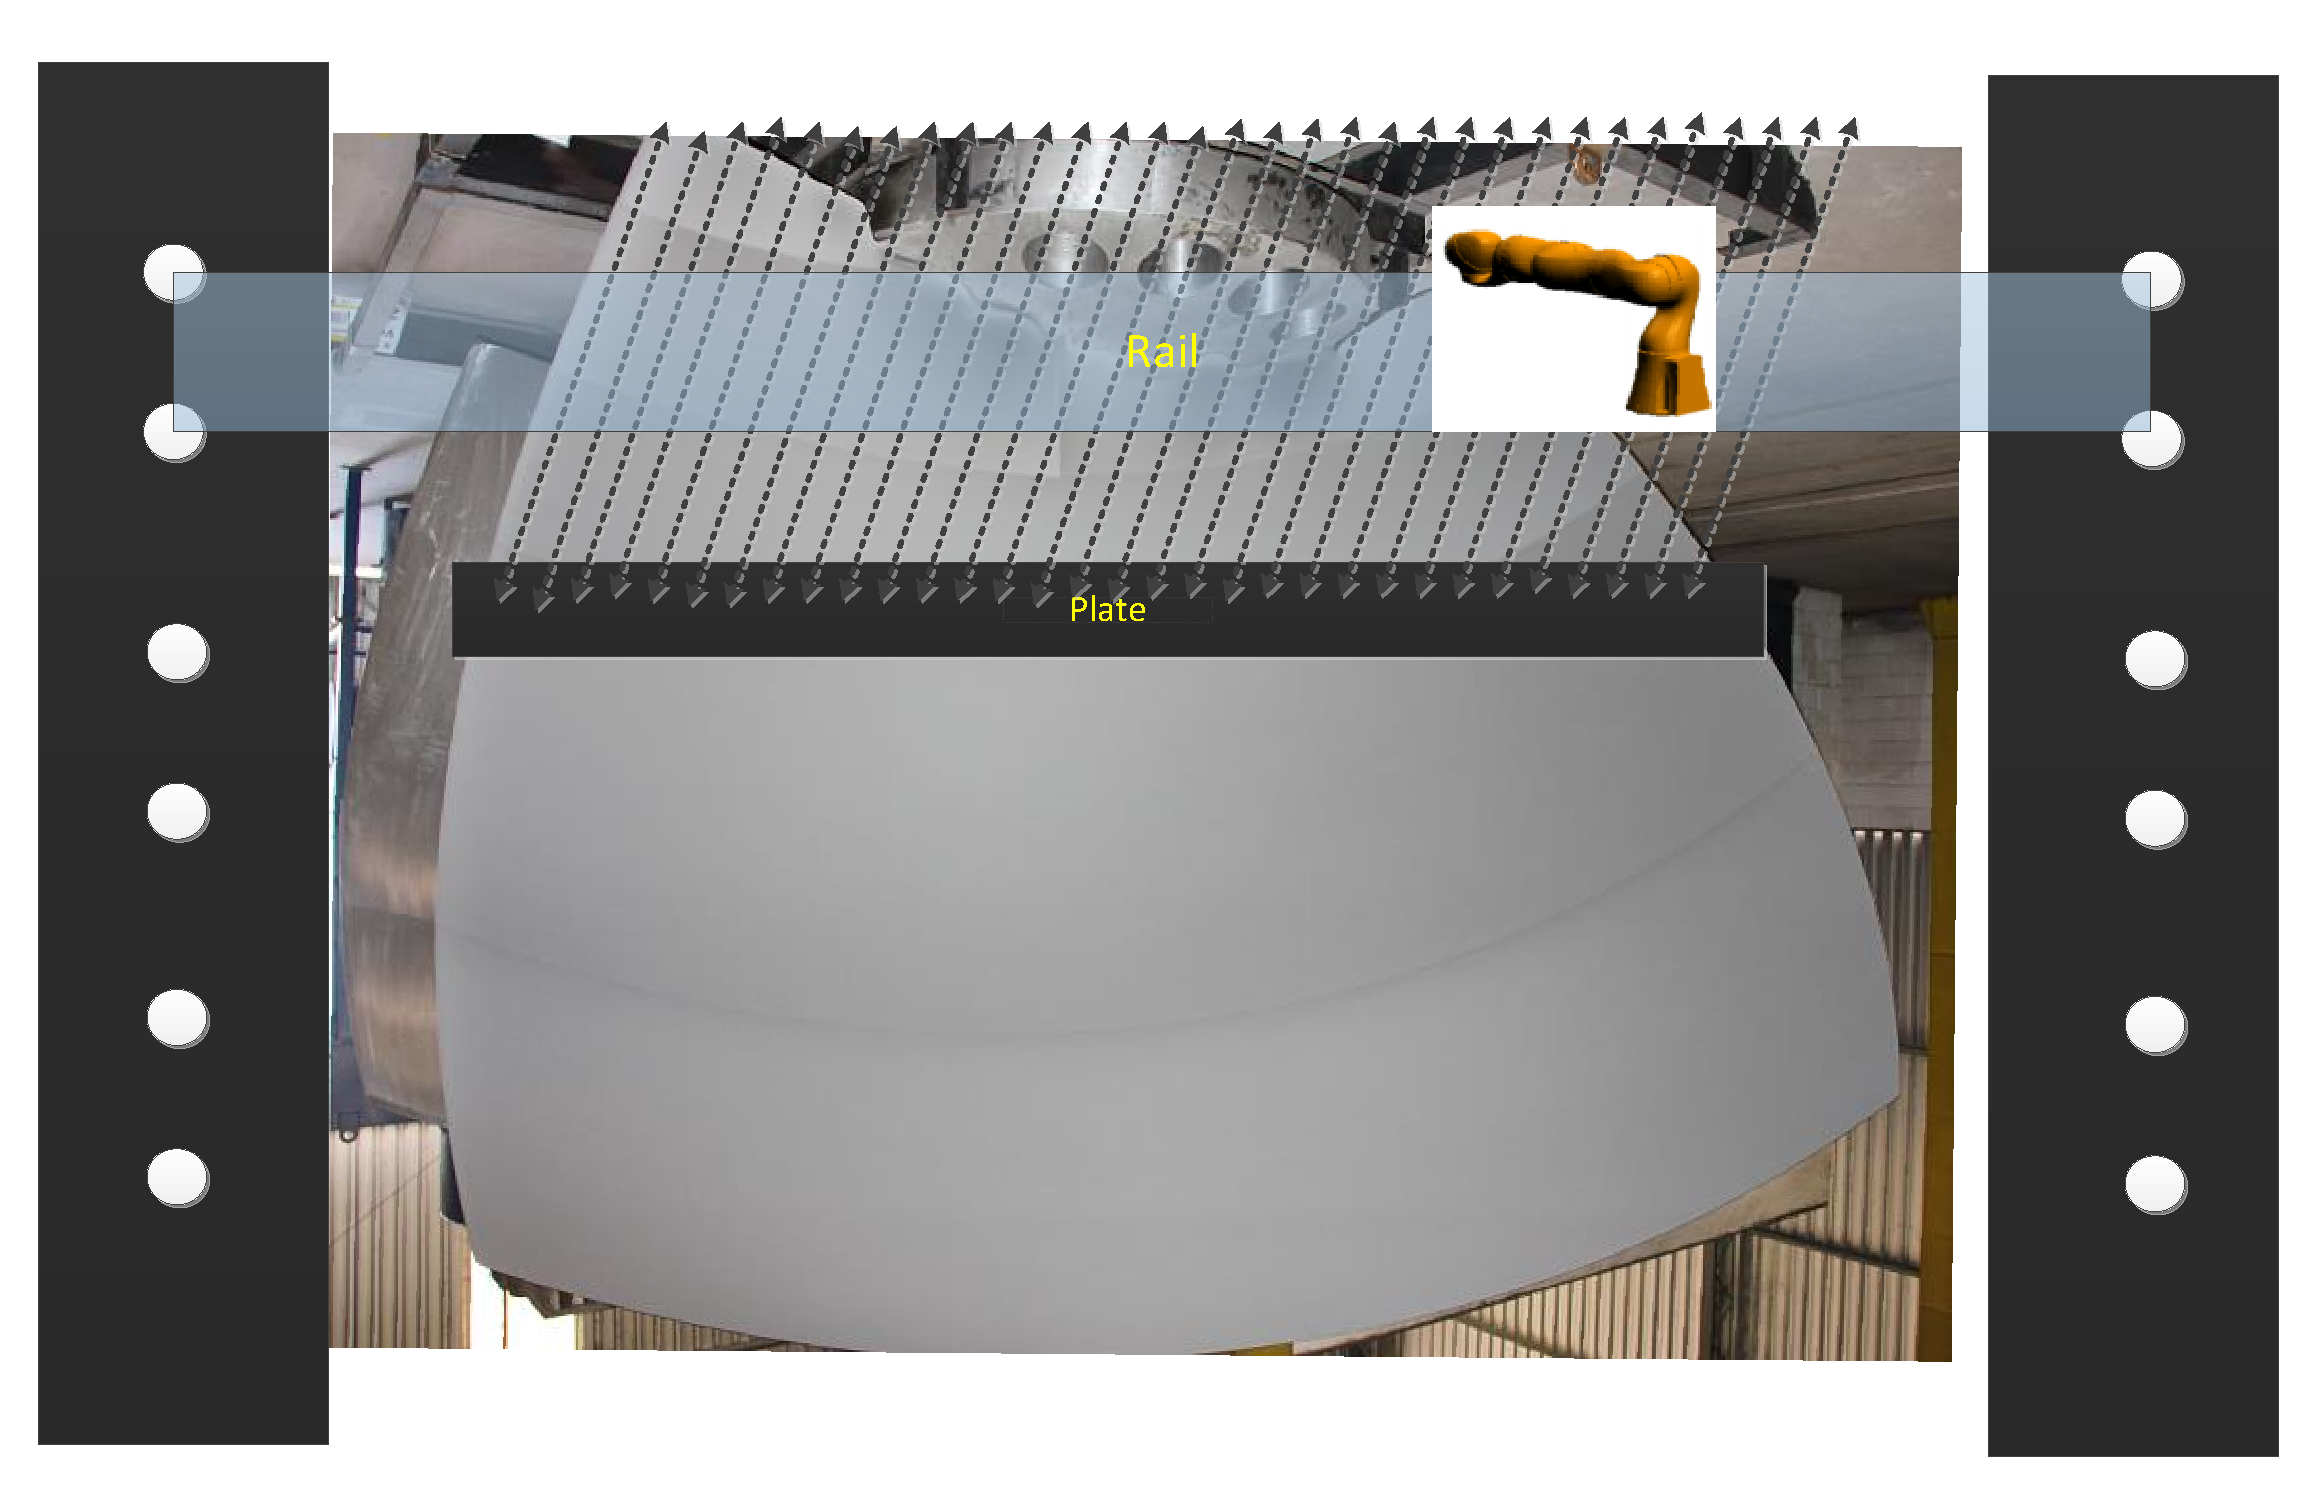
\includegraphics[width=\columnwidth]{figs/trilhos/rail2.pdf} 
	\caption{Trilho fora da pá com processamento em diagonal.}
	\label{rail2}
\end{figure}

Esse tipo de abordagem simplifica a movimentação do robô no
trilho, uma vez que o trilho seria totalmente reto, e possibilitaria a
metalização de um dos lados das quatro pás com uma única instalação de base.
Porém, mesmo nesta solução, a altura do trilho deverá ser ajustada três vezes para
cada lado de pá, e toda a estrutura deverá ser reinstalada no outro lado da
turbina para a realização do processo no outro lado das pás.

Em ambos os sistemas propostos, é necessária a implementação de um sistema de
localização do robô em relação à pá, tornando possível a geração de um
planejamento de trajetórias para o processo de metalização. O sistema de
localização pode ser concebido por sensores externos
ao robô (câmeras e outros), ou instalados no próprio manipulador/base.

\textbf{Conclusão da solução por robôs em trilhos}
A solução com trilho externo se mostrou vantajosa em comparação ao robô em
trilho customizado acoplado à pá, devido à complexidade e intervenções
manuais. Há a possibilidade de utilizar um manipulador industrial, tornando o
foco do projeto em processamento de sinais, mapeamento, localização e controle,
além da construção do trilho. Porém, a montagem da estrutura e a instalação de
todo o sistema atrás da pá podem ser custosas, sendo esta ainda uma solução
considerada complexa.
\subsection{Projeto de robôs escaladores}\label{proj_climbers}
% "scan" use succion-based mobile system (ICM climber) and place an arm on it.
% Is blade is above maximal curvature ?
% rail em movimento
Nesta subseção, consideram-se soluções para HVOF de pás de turbinas robôs
escaladores com fusão das tecnologias documentadas na
seção~\ref{sota}, subseção~\ref{sota_climbers}.

A solução mais completa, que mais atendia às especificações e possibilita
aperfeiçoamento 
\subsubsection{Projetos com manipuladores industriais fixos}\label{proj_manip}
Há diversos manipuladores robóticos industriais com as especificações
necessárias para a realização da tarefa de metalização por HVOF. As empresas
Fanuc, Motoman, ABB e KUKA fabricam manipuladores com dimensões compatíveis com o
acesso pela escotilha inferior e velocidade, precisão, e espaço de trabalho que
cumprem os requisitos para a execução do processo em todo um lado da pá, em uma
base fixa. Porém, há a necessidade de escolher a posição correta do manipulador
em relação à pá, a fim de maximizar a sua área de trabalho, no ambiente da
turbina, o que pode restringir os seus movimentos.
Como as pás podem ser giradas até um ângulo de $14.5^o$, são discutidas as ideias de posicionamento
do manipulador entre as pás, a fim de executar a operação em ambos os lados da
pá (um lado de cada pá), e o posicionamento fixo à frente da pá.

\textbf{Posicionamento entre pás}
A figura~\ref{fig::andaime} mostra o espaço entre as pás da turbina, dentro do
aro câmara. Um robô manipulador de médio porte pode ser fixado em uma base
magnética, na posição que se encontra a escada da figura~\ref{fig::andaime}.
Essa posição é vantajosa por possibilitar a execução da tarefa em duas pás
(frente de uma e verso da outra), sem desmontar ou fazer grandes alterações no
posicionamento da base do robô, diminuindo as intervenções e tempo de tarefa.

O estudo puramente geométrico demonstra que o alcance do manipulador robótico
para o processamento de ambos os lados das pás, considerando uma base fixa entre
as pás, deverá ser em torno de 5 metros. O manipulador industrial IRB5500,
desenvolvido pela ABB para pintura, possui 3 metros de alcance, porém 180 kg, o que já dificulta ou até impossibilita a
logística de movimentação e posicionamento in-situ. Não foi encontrado um robô
industrial com o alcance necessário e que tivesse as dimensões máximas da
escotilha inferior. 

A solução conceitual de posicionar um manipulador industrial entre as pás deve
avaliar, portanto, todas as configurações necessárias da base (orientações e
posições) para garantir que todo o espaço de trabalho do manipulador mais base
cubra os lados de ambas as pás. O número de configurações e o projeto
mecânico da base são extremamente necessários para a viabilização da solução,
uma vez que será possível avaliar as intervenções e complexidades. Bases
autônomas diminuem o número de intervenções e aumentam a precisção do sistema,
porém aumentam a complexidade, o custo devido ao número de sensores e atuadores
e o peso do sistema, prejudicando a logística.

\textbf{Posicionamento à frente da pá}
Posicionar de maneira fixa um manipulador com base magnética à frente da pá para
a metalização é uma solução natural, já que é semelhante à utilizada pela
empresa Rijeza atualmente. Um estudo puramente geométrico, utilizando as
dimensões da pá, mostra que o manipulador deve possuir alcance de 1.7 m e ser
posicionado a uma altura de 1.1 m em relação ao solo. Estudos de espaço de
trabalho, manipulabilidade e colisões devem ser realizados para confirmar o
estudo geométrico.

O posicionamento do sistema à frente da pá exige intervenções para rotação da
turbina e para o deslocamento do sistema para trás da pá. Em relação a um
sistema com base autônoma entre as pás, o processo parece mais custoso em
intervenções manuais e mais demorado, porém bem mais simples.

\textbf{Conclusão da solução com manipuladores industriais}
A utilização de manipuladores industriais é a mais simples dentre todas as soluções para o acesso pela escotilha inferior. Não há projeto mecânico
do manipulador, já que este será adquirido em um dos fabricantes citados. As
dificuldades mecânicas do projeto serão em relação à logística de posicionamento
e movimentação do robô dentro do aro câmara, e no desenvolvimento de uma base,
que pode ser autônoma. Além disso, o projeto fica responsável pelo controle do
manipulador, processamento de dados que envolvem o HVOF, planejamento de
trajetórias e UI.

Este projeto conceitual será uma das frentes para o estudo de viabilidade.
 
% RIWEA-like rail on which the coating system
%  place blade horizontal and use wheels, against the blade's rim,to move a rail
  % along the blade's shape
  %  two-arm solution (or one arm + magnetic attachment point) to allow reaching
  % the top of the blade from the very bottom
\subsection{Robô Bipartido}

Esse conceito é uma cadeia de dois manipuladores conectados por um ponto de
apoio capaz de fixar-se à pá. O apoio serve como forma reduzir o torque
necessário nas juntas ao reduzir a alcance necessário para cada manipulador
individualmente.

Para facilitar futuras referências nesse texto, o braço robótico que se
apoia sobre o chão será chamado de primário, manipulador que parte dele de
secundário e o ponto de apoio entre eles, capaz de fixa-se à pá, será chamado de
fixador.

 A pistola de metalização presa ao manipulador secundário deve ter
alcance sobre toda a pá da turbina. Para isso existe uma gama de pontos
necessários onde o fixador deve ser posicionado. Com esse intuito o
manipulador primário da cadeia precisa ser projetado para ter uma região de
trabalho com um alcance total sobre esses pontos. Para tal, informações precisas
sobre o formato das pás são necessárias.

Para viabilizar a solução, é necessário verificar quais são as soluções
possíveis para gerar a aderencia do fixador sobre à pá. As tecnologias mais
difundidas são por força magnética e por diferença de pressão (ventosa).
As maiores preocupações com o relação a adesão são a capacidade de carga do
método e a resistência do \textit{coating}. As soluções por magnetismo e
por ventosa afetam de maneira diferente as camadas do material ao qual se
aderem. Enquanto o magnetismo atrai ativamente o material ao qual prentende
aderir, a ventosa apenas reduz a pressão do ar na região onde ela se fixa. Ambas
as soluções possuem versões ativas e passivas, assim como uma gama de opções com
relação à capacidade de suportar carga. Logo, para essas soluções, a carga
necessária a ser suportada, o magnetismo do material, a resistência à baixa
pressão do \textit{coating} e os efeitos da atração magnética, também, sobre o
\textit{coating} são perguntas que devem ser respondidas.

O braço secundário deve ser projetado para atingir os requerimentos de
posicionamento e velocidade da pistola de metalização, porém a região sob o
fixador, certamente, não estará disponivel para receber o revestimento. Assim, a
possibilidade, ou os requisitos necessários, de mover o fixador para uma região
da pá recém metalizada deve ser vista analisada antes do robô bipartido ser
considerado uma possibilidade.

\subsection{Robô Pendurado} 


 % attach a rail to the blade and move it manually
 
 % attach a rail one the nose and ground, 1D movement and move the blade to
 

\subsection{Projeto de robôs escaladores}\label{proj_climbers}
% "scan" use succion-based mobile system (ICM climber) and place an arm on it.
% Is blade is above maximal curvature ?
% rail em movimento
Nesta subseção, consideram-se soluções para HVOF de pás de turbinas robôs
escaladores com fusão das tecnologias documentadas na
seção~\ref{sota}, subseção~\ref{sota_climbers}.

A solução mais completa, que mais atendia às especificações e possibilita
aperfeiçoamento 
 
% RIWEA-like rail on which the coating system
%  place blade horizontal and use wheels, against the blade's rim,to move a rail
  % along the blade's shape
  %  two-arm solution (or one arm + magnetic attachment point) to allow reaching
  % the top of the blade from the very bottom
\subsection{Robô Bipartido}

Esse conceito é uma cadeia de dois manipuladores conectados por um ponto de
apoio capaz de fixar-se à pá. O apoio serve como forma reduzir o torque
necessário nas juntas ao reduzir a alcance necessário para cada manipulador
individualmente.

Para facilitar futuras referências nesse texto, o braço robótico que se
apoia sobre o chão será chamado de primário, manipulador que parte dele de
secundário e o ponto de apoio entre eles, capaz de fixa-se à pá, será chamado de
fixador.

 A pistola de metalização presa ao manipulador secundário deve ter
alcance sobre toda a pá da turbina. Para isso existe uma gama de pontos
necessários onde o fixador deve ser posicionado. Com esse intuito o
manipulador primário da cadeia precisa ser projetado para ter uma região de
trabalho com um alcance total sobre esses pontos. Para tal, informações precisas
sobre o formato das pás são necessárias.

Para viabilizar a solução, é necessário verificar quais são as soluções
possíveis para gerar a aderencia do fixador sobre à pá. As tecnologias mais
difundidas são por força magnética e por diferença de pressão (ventosa).
As maiores preocupações com o relação a adesão são a capacidade de carga do
método e a resistência do \textit{coating}. As soluções por magnetismo e
por ventosa afetam de maneira diferente as camadas do material ao qual se
aderem. Enquanto o magnetismo atrai ativamente o material ao qual prentende
aderir, a ventosa apenas reduz a pressão do ar na região onde ela se fixa. Ambas
as soluções possuem versões ativas e passivas, assim como uma gama de opções com
relação à capacidade de suportar carga. Logo, para essas soluções, a carga
necessária a ser suportada, o magnetismo do material, a resistência à baixa
pressão do \textit{coating} e os efeitos da atração magnética, também, sobre o
\textit{coating} são perguntas que devem ser respondidas.

O braço secundário deve ser projetado para atingir os requerimentos de
posicionamento e velocidade da pistola de metalização, porém a região sob o
fixador, certamente, não estará disponivel para receber o revestimento. Assim, a
possibilidade, ou os requisitos necessários, de mover o fixador para uma região
da pá recém metalizada deve ser vista analisada antes do robô bipartido ser
considerado uma possibilidade.

\subsection{Robô Pendurado} 

\subsection{Acesso pela jusante}
%TODO Abelha: prós e contras do acesso, soluções, apresentar soluções de
% logística


Como última opção de acesso ao rotor existe a possibilidade de utilização do
tubo de sucção ou descarga como meio de entrada à turbina. Com o fluxo de água
parado, é possível utilizar o Rio como meio de lançamento do sistema. A
complexidade da operação para utilizar esse acesso é maior, entretanto existem
vantagens que podem tornar essa solução possível e mais atrativa.

\textbf{Vantagens}
\begin{itemize}
  \item Virtualmente nenhuma restrição de tamanho
  \item Flexibilidade de soluções
  \item Facilidade de utilização de um manipulador industrial \textit{standard}
  \item Possibilidade de implementação em outras usinas
\end{itemize}

\textbf{Desvantagens}
\begin{itemize}
  \item Complexidade de lançamento e recuperação
  \item Custo
  \item Possibilidade de correnteza
  \item Complexidade logística de transporte entre a entrada do tubo de sucção e
  o aro câmara
  \item Complexidade de prototipação
\end{itemize}

As possíveis soluções foram divididas nas etapas necessárias para a operação, ou
seja, lançamento e recuperação do sistema, logística de transporte e o robô de
metalização propriamente dito.

Para esse acesso, o maior obstáculo presente é o desenvolvimento de um sistema
de lançamento e recuperação do robô, a partir do rio, até o interior da turbina.
Essa operação deverá ser realizada com a turbina alagada e, em seguida, deverá
ser realizada a drenagem da mesma. É importante que o sistema de lançamento seja
robusto e garanta o perfeito posicionamento do robô dentro da turbina, assim
como, a sua recuperação. Uma vez que o sistema não pode se perder no leito do
rio.

Primeiramente, o sistema deve ser a prova d'água com classificação de pelo
menos 50m.
Sendo assim, um vaso de pressão para o transporte do robô até o interior da turbina deve ser
desenvolvido, não havendo necessidade do maniupuladore responsável pela
metalização em si ser a prova d'água. O \textit{container} de transporte
submarino deve ser menor que o tamanho do vão do stoplog, uma vez que ele
utilizirá esse caminho para acessar o tubo de descarga. Por outro lado, deve ser
grande o suficiente para o robô e todo o material necessário seja transportado e
também que suporte uma escotilha de acesso de tamanho suficiente para que todo o
sistema seja retirado do seu interior.

Para o sistema de lançamento foi deslumbrada uma estrutura de transporte que
utilizará o pórtico rolante e o trilho guia dos stoplogs. Após a submersão da
estrutura, um mecanismo de lançamento, inspirado em um paletizador, é
responsável pelo posicionamento do \textit{container} sempre no mesmo ponto em
relação ao tubo de descarga. Com o vaso de pressão posicionado, a turbina deve
ser, então, drenada. Com a turbina seca, o robô pode ser retirado de seu
envólucro e a operação de metalização pode ter seu início. Uma etapa crítica da
operação é a recuperação do sistema, na qual a turbina deve ser novamente
alagada e os os stoplogs retirados. Em seguida, a estrutura de transporte deve
recuperar o \textit{container} transportador na mesma posição em que o sistema
foi lançado. O sucesso dessa operação tem como \textbf{hipótese que a velocidade
de drenagem e a correnteza gerada por essa operação não são suficientes para
retirar o container (mais pesado que a água) de sua posição inicial}. 

A movimentação do robô do ponto de lançamento até o aro câmara deverá ser
realizada a partir da utilização de cordas, roldanas e talhas. Caso necessário,
pode ser desenvolvido um sistema de locomoção com trilhos e/ou rodas atuadas
para o posicionamento automático do robô.

O robô de metalização pode ter diversos fomatos, mas devido a possilidade de se
utilizar um manipulador industrial padrão, o projeto inicial consiste em uma
base de apoio e um manipulador com alcance para o processmento de uma face da pá
posicionado de frente para pá, ou um manipulador posicionado entre duas pás com
alcance de para processar as duas as faces das pás voltadas para ele.

\subsubsection{Dimensionamento da base}

Para manipuladores com longo alcance, as forças e torques envolvidos requerem
uma estrutura de fixação do robô de forma que o sistema como um todo não se
movimente e, no caso extremo, tombe. Normalmente, os manipuladores robóticos são
fixados no chão e as características da superfície e dos parafusos são
estipulados pelo fornecedor a partir dos valores máximos de torque e força que o
manipulador exerce em sua base. Para uma base apoiada no chão, dois fatores
influenciam capacidade de estabilização da estrutura: o raio da base e o seu
peso.

O raio da base $r_{b_f}$ é limitado pelo ambiente da turbina e para cada
posicionamento existem restrições específicas. 
Para a realização dos cálculos de dimensionamento foi considerado,
primeiramente, o manipulador posicionado em frente a pá e processando somente uma face por vez
e a uma altura de 1000mm, posição em que o alcance necessário do robô é de
1800mm. Para essas características, o tamanho máximo que a base pode assumir é
de aproximadamente 1600mm, caso a estrutura seja projetada de forma a seguir os contornos do aro câmara.
A figura \ref{fig::base_aro_frente} %TODO figura base_aro_frente
representa um esboço da vista frontal do aro câmara e a largura máxima que a
base pode assumir. A análise da dimensão máxima da base no sentido paralelo ao
fluxo da água pode ser realizada com o auxílio do desenho técnico fornecido pela
ESBR, ilustrado na figura \ref{fig::turbine_side}. O limite superior nessa
região é determinado pela transição do aro câmara para a região inclinada do
tubo de sucção e é de aproximadamente 1600mm. Entrentanto esse limite pode ser
contornado construindo-se um plano horizontal ou projetando-se a base de forma que ela acompanhe essa
inclinação. Ao se incluir o dimensionamento da base no cálculo do alcance mínimo
do manipulador deve ser realizado uma alteraçao, uma vez que agora o manipulador
se encontra deslocado da superfície da pá. Sendo assim, alcance mínimo se
relaciona com o tamanho do raio da base de acordo com
$$a_{min}=\sqrt{r_b^2+1800^2}.$$

O cálculo das dimensões da base com o robô posicionado dentro do aro câmara e
entre as pás depende do angulo de ataque das pás e do cálculo do ângulo diédrico
entre elas. A amplitude do movimento de rotação $alpha$ das pás é de $14,5^o$
para cada lado a partir da posição zero, entretanto \textbf{essa posição não pôde ser
informada no momento da viagem de reconhecimento e ainda não foi
disponibilizada}. Para critério de cálculos foi utilizado um ângulo de
$45^o$ como a posição de maior abertura das pás e o zero foi considerado como
a reta perpendicular ao fluxo de água. O ângulo diédrico $\theta$ entre as pás depende da rotação
sofrida pelas mesmas e obedece a relação $\cos{\theta} = \sin^2{\alpha}.$

O arco de circunferência pode ser obtido a partir da relação $arc=R*\alpha$ com
R=3850mm. O raio máximo da base pode ser calculada como 
$$r_{b_e} = (R - h_{b_e})\tan{\theta/2},$$  ilustrado na figura
\ref{fig:calc_base_entre} e com $h_{b_e}$ sendo a altura da base.

O peso mínimo que a base do robô deve possuir está diretamente relacionada com o
tamanho de seu raio. A firgura \ref{fig::tilt_robot} faz uma representação
simplificada da forma que o torque de capotamento máximo atua no robô e em sua
base. Na situação limite, considerando o torque com sentido horário, a força
normal entre a base e a superfície de apoio $N_2$ teria módulo igual a zero.
Considerando o pior caso, ou seja, a força vertical que o robô exerce na base é
composta apenas pelo seu peso $W$ para que a base não se mova durante a
operação, temos que o somatório das forças e torques sejam iguais a zero.

A análise das forças nos fornece que $N_1$ tenha módulo igual ao peso do robô e
o somatório dos torques se reduz a $M_k-Wr_b=0$. Sendo assim, a relação entre
o raio da base, seu peso e o torque máximo de capotamento exercido pelo robô é
da forma 

$$M_k=Wr_b.$$

%TODO refazer figura
\begin{figure}[h!]
\centering
	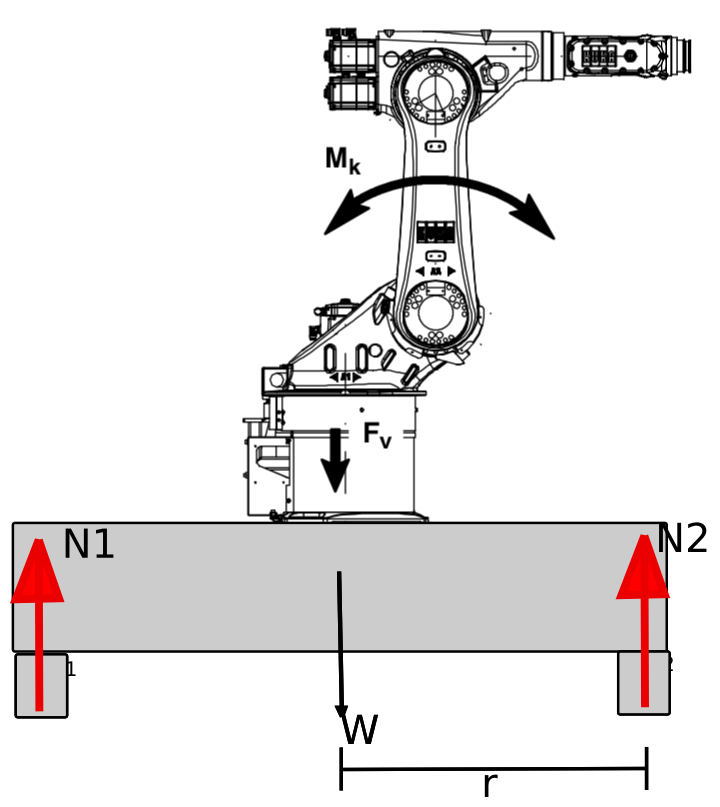
\includegraphics[width=0.5\columnwidth]{figs/base/tilt}
	\caption{Forças e torques máximos entre o robô e sua base.}
\end{figure}

Uma vez que a superfície do aro câmara e a região adjacente no tubo de sucção
são \textbf{ferromagnéticas}, é possível a utilização de bases magnéticas para
uma compensação do peso e raio necessário para a estabilização do robô. Os
dispositivos magnéticos se dispõem de duas maneiras para essa aplicação:
eletretromagnéticos e imãs permanentes. O primeiro caso tem como principal
vantagem a possibilidade de acionamento remoto, entretanto para situações de
falha em que haja perda de fornecimento de energia a força de atração também é
perdida. O segundo caso consiste em imãs permanentes arrumados de maneira que
seja possível organizar o fluxo magnético e, assim, controlar por meio de uma
alavanca a presença ou ausência de força magnética. A figura
\ref{figs/base/imas} ilustra os dois tipos de bases magnéticas citados.
Comercialmente, foram encontrados bases magnéticas com capacidade de até 3000N.

%TODO figura imãs













\section{Resultados do estudo}\label{sec:resultados}
%TODO
\section{Conclusão e trabalhos futuros}\label{sec:conclusions}
  
\bibliography{main} 
\appendix
\end{document}
